\documentclass[conference]{IEEEtran}

\usepackage{cite}
\usepackage{amsmath,amssymb,amsfonts}
\usepackage{graphicx}
\usepackage{textcomp}
\usepackage{xcolor}
\usepackage{booktabs}
\usepackage{array}
\usepackage{url}

\graphicspath{{figures/}}
\newcommand{\reporttablesize}{\footnotesize}
\newcommand{\singlefigwidth}{0.98\linewidth}
\newcommand{\widefigwidth}{0.96\textwidth}

\def\BibTeX{{\rm B\kern-.05em{\sc i\kern-.025em b}\kern-.08em
    T\kern-.1667em\lower.7ex\hbox{E}\kern-.125emX}}

\begin{document}

\title{Causal Emotion Geometry in a Fine-Tuned Speech Model: An Anthropic-Inspired Study of Direction Steering and Activation Patching}

\author{
\IEEEauthorblockN{Pavan Nadendla}
\IEEEauthorblockA{\textit{Data Science Final Project} \\
\textit{California State University, Los Angeles}\\
Los Angeles, United States}
}

\maketitle

\begin{abstract}
This project begins as a speech emotion recognition system and ends as a small mechanistic interpretability study. Inspired by Anthropic's work on emotion concept vectors in large language models, we ask whether a speech model only learns to map acoustic features to an emotion label, or whether its hidden states also contain manipulable internal emotion representations that help cause the final prediction. We fine-tune \texttt{facebook/wav2vec2-base} on a speaker-independent six-class RAVDESS task and compare it against a mel-spectrogram CNN baseline. wav2vec2 reaches 0.8269 test accuracy and 0.8126 macro F1, compared with 0.4231 accuracy and 0.3241 macro F1 for the CNN. We then build emotion-minus-neutral directions in wav2vec2 hidden space. A direction-only prototype classifier using actor/statement-controlled directions reaches 0.8413 accuracy and 0.8301 macro F1 on held-out speakers, while shuffled-label directions collapse to 0.0151 macro F1 in the direct control. The causal results are the core contribution: projection onto an emotion direction correlates with the model's probability for that emotion; adding a direction raises target probability; removing all non-neutral direction components drops macro F1 by -0.2889 with a bootstrap 95\% CI of [-0.3395, -0.2487]; and norm-matched random directions do not reproduce this effect. Mid-transformer direction injection works inside wav2vec2 itself, with the strongest average sufficiency effect at layer 7 (+0.2545 target probability at alpha 0.5). Finally, same-context activation patching transfers emotion identity from source clips to destination clips: at layer 11, source-emotion probability rises by +0.6796 (95\% CI [0.6475, 0.7092]) and the prediction flips to the source emotion in 75.62\% of controlled pairs. The final claim is functional, not anthropomorphic: the model does not feel emotion, but it carries emotion as a causal internal representation that can be measured, steered, removed, and patched to change outputs.
\end{abstract}

\begin{IEEEkeywords}
speech emotion recognition, wav2vec2, mechanistic interpretability, causal intervention, activation patching, emotion directions, RAVDESS
\end{IEEEkeywords}

\section{Introduction}

A standard speech emotion recognition (SER) project asks whether a model can classify audio into labels such as neutral, happy, sad, angry, fearful, and disgust. That is useful, but it leaves the most interesting question untouched: after the model learns the task, what kind of internal representation actually carries the answer?

The framing of this project is that a model may learn two related things at once. First, it learns predictive features that allow a classifier head to output an emotion class. Second, it may organize those features into internal concept directions or subspaces corresponding to emotion-like variables. If those internal variables are real parts of the computation, then changing them should change the model's output.

This is the bridge to Anthropic's recent work on emotion concepts in Claude Sonnet 4.5 \cite{sofroniew2026emotion}. Anthropic extracted linear emotion vectors from internal activations using labeled synthetic stories, validated that those vectors activate in appropriate emotional contexts, and showed that interventions on those vectors can affect model behavior. Their work is careful about interpretation: the existence of functional emotion representations does not imply subjective feeling. Instead, it shows that emotion concepts can be represented internally and can shape behavior.

Our project translates that idea into speech. The model is not a conversational LLM, so we cannot study generated text, preferences, or Assistant behavior. Instead, we deliberately choose a speech emotion prediction task where the output is a probability distribution over emotion classes. This gives us a cleaner measurement target: if an internal ``angry minus neutral'' direction is meaningful, projection onto it should correlate with angry probability, injecting it should raise angry probability, removing it should hurt angry recognition, and patching hidden states from an angry clip into another clip should transfer angry evidence.

The SER setting is also intentionally conservative. Prior SER work has emphasized that emotion recognition can be fragile under different splits, corpora, and feature pipelines \cite{schuller2009emotion,khalil2019serreview,lieskovska2021attentionreview}. For that reason, we treat speaker independence, shuffled-label controls, random-vector controls, and cross-dataset transfer as part of the claim rather than as optional evaluation details.

\section{Dataset and Models}

The project uses the RAVDESS audio-only speech subset \cite{livingstone2018ravdess}. The original speech set contains 1,440 clips. The final six-class task keeps 1,248 clips after mapping calm into neutral and dropping surprised.

\begin{table}[t]
\caption{Final RAVDESS Six-Class Dataset}
\label{tab:dataset}
\centering
\reporttablesize
\begin{tabular}{@{}lc@{}}
\toprule
\textbf{Class} & \textbf{Count} \\
\midrule
neutral & 288 \\
happy & 192 \\
sad & 192 \\
angry & 192 \\
fearful & 192 \\
disgust & 192 \\
\midrule
total & 1248 \\
\bottomrule
\end{tabular}
\end{table}

The split is speaker-independent: actors 01--16 are used for training, actors 17--20 for validation, and actors 21--24 for testing. This prevents speaker memorization from inflating performance and creates a stronger setting for interpretability.

The main model fine-tunes \texttt{facebook/wav2vec2-base} \cite{baevski2020wav2vec2}, a pretrained self-supervised transformer-style raw speech encoder \cite{vaswani2017attention}, with a classification head. The comparison baseline is a CNN trained on log-mel spectrograms. Table \ref{tab:model_comparison} shows the supervised performance.

\begin{table}[t]
\caption{Supervised Model Comparison}
\label{tab:model_comparison}
\centering
\reporttablesize
\begin{tabular}{@{}lccc@{}}
\toprule
\textbf{Model} & \textbf{Split} & \textbf{Accuracy} & \textbf{Macro F1} \\
\midrule
wav2vec2 & val & 0.7885 & 0.7762 \\
wav2vec2 & test & 0.8269 & 0.8126 \\
CNN & val & 0.4375 & 0.3722 \\
CNN & test & 0.4231 & 0.3241 \\
\bottomrule
\end{tabular}
\end{table}

\begin{figure}[t]
\centering
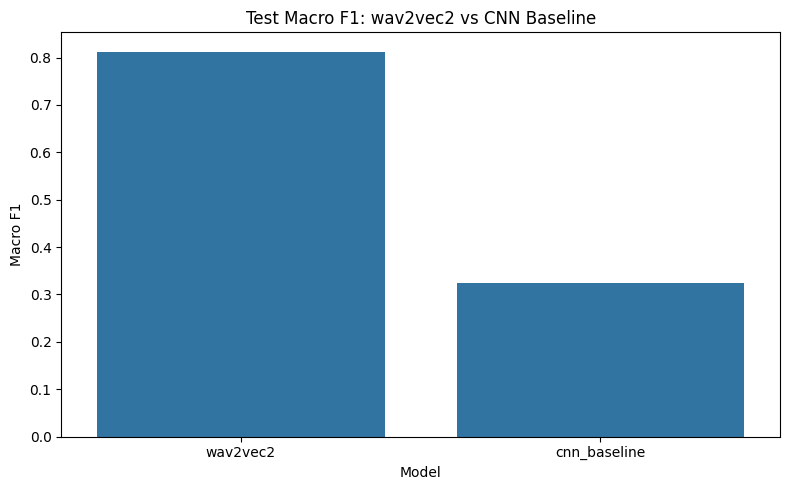
\includegraphics[width=\singlefigwidth]{06_model_comparison_cell_04_fig_01_model_comparison.png}
\caption{wav2vec2 strongly outperforms the mel-spectrogram CNN baseline on held-out speakers.}
\label{fig:model_comparison}
\end{figure}

The gap is large: wav2vec2 improves test macro F1 by 0.4885 over the CNN. This establishes the predictive foundation. The remaining experiments ask what that predictive ability is made of internally.

\section{Anthropic-Inspired Method}

Anthropic's setup can be summarized as: extract concept vectors from activations, verify that they activate in relevant contexts, and intervene on them to test whether they influence behavior. Our speech version follows the same logic with a different model, modality, and output. This intervention-first framing is also connected to broader mechanistic interpretability work on transformer circuits and causal model analysis.

For a pooled hidden-state embedding $z_i$, we compute class centroids from training embeddings. Using neutral as the reference class, an emotion direction is:

\begin{equation}
d_c = \mu_c - \mu_{\mathrm{neutral}}.
\end{equation}

For a sample embedding $z$, the scalar projection onto direction $d_c$ is:

\begin{equation}
p_c(z) = z \cdot \frac{d_c}{\lVert d_c \rVert}.
\end{equation}

We also build controlled versions of these directions by centering embeddings within actor and statement groups before computing centroids. This makes the direction closer to ``emotion after removing speaker/sentence confounds'' rather than ``emotion mixed with who spoke or what sentence was spoken.''

\begin{figure*}[t]
\centering
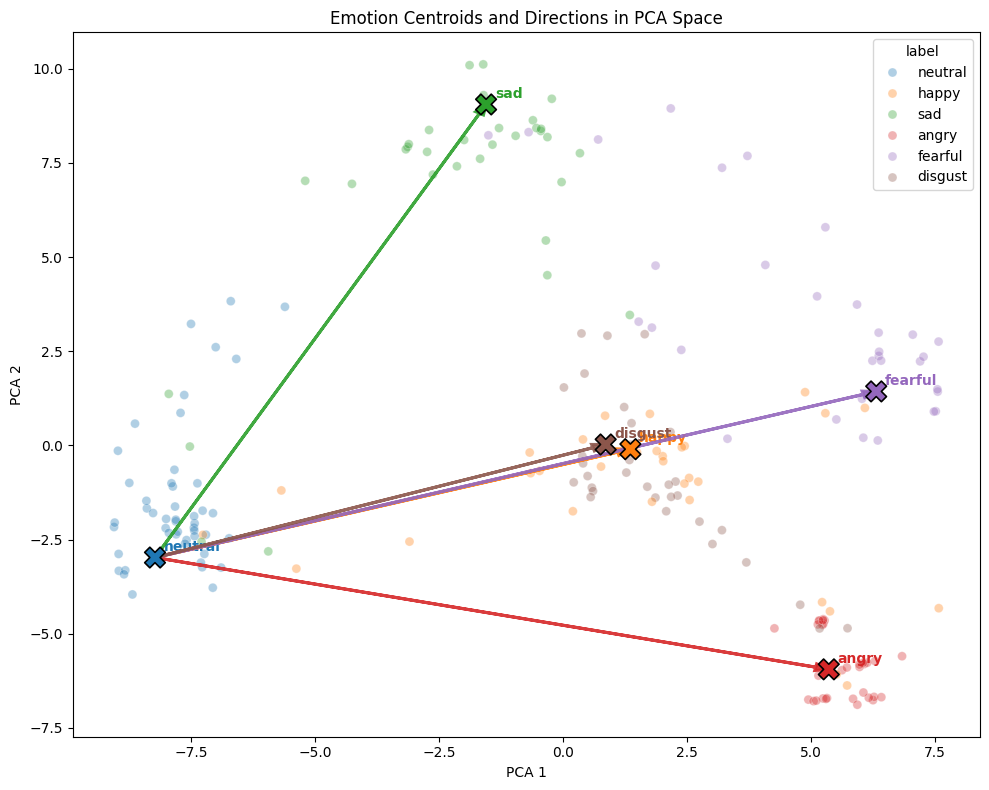
\includegraphics[width=0.72\textwidth]{07_anthropic_style_emotion_vectors_cell_09_fig_06_anthropic_style_emotion_vector_analysis.png}
\caption{Emotion centroids and neutral-to-emotion directions visualized in PCA space. This figure gives the report's geometric intuition: emotion classes form structured regions, and directions from the neutral centroid point toward emotion-specific regions.}
\label{fig:emotion_centroids}
\end{figure*}

We test these directions in an increasingly causal sequence: direction-only classification, projection-probability correlation, steering, ablation, mid-transformer intervention, activation patching, and negative controls. This progression is the main story of the project: we move from a classifier, to latent geometry, to causal intervention.

\section{Predictive Emotion Geometry}

\subsection{Direction-Only Prototype Classification}

A direction-only classifier predicts emotion using projections onto the learned emotion directions. With actor/statement-controlled directions, it reaches 0.8413 test accuracy and 0.8301 macro F1. The trained classifier head in the same embedding analysis reaches 0.8365 accuracy and 0.8237 macro F1.

\begin{table}[t]
\caption{Direction-Only Prototype Classification}
\label{tab:direction_only}
\centering
\reporttablesize
\begin{tabular}{@{}lcc@{}}
\toprule
\textbf{Method} & \textbf{Accuracy} & \textbf{Macro F1} \\
\midrule
raw directions & 0.8365 & 0.8255 \\
controlled directions & 0.8413 & 0.8301 \\
shuffled-label directions & 0.0192 & 0.0151 \\
trained head & 0.8365 & 0.8237 \\
\bottomrule
\end{tabular}
\end{table}

\begin{figure}[t]
\centering
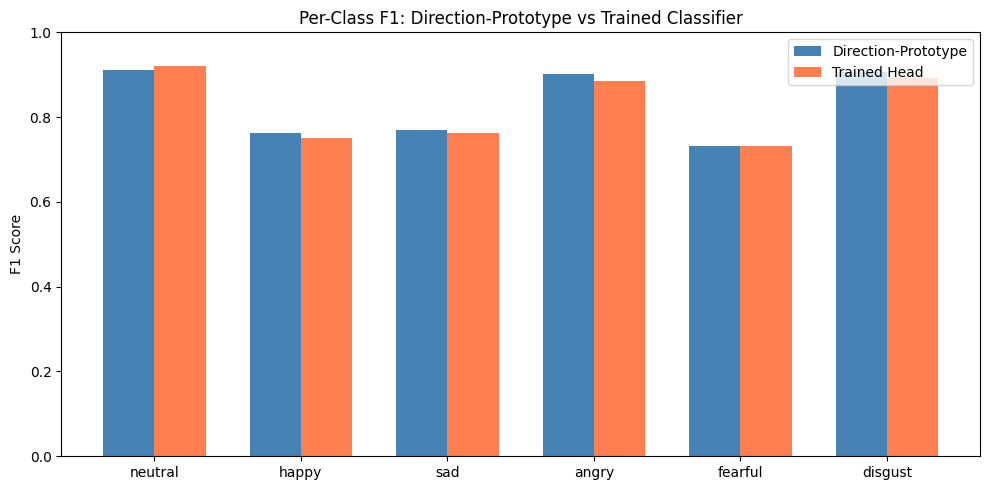
\includegraphics[width=\singlefigwidth]{08_direction_only_classification_cell_06_fig_01_direction_only_vs_trained_classifier.png}
\caption{Per-class F1 for the controlled direction-only classifier and trained classifier head.}
\label{fig:direction_f1}
\end{figure}

This result shows that the hidden space is not an uninterpretable cloud where only the classifier head knows the answer. A small set of emotion directions recovers essentially all of the supervised classifier's behavior. The shuffled-label control prevents a weak interpretation: arbitrary centroid directions do not work.

\subsection{Projection Magnitude Tracks Probability}

If a direction is truly related to an emotion concept in the model, then higher projection onto that direction should mean higher predicted probability for that emotion. Across all test samples, Pearson correlations between direction projection and target probability range from 0.6812 to 0.7711. Within true-class subsets, correlations range from 0.6701 to 0.9525.

\begin{figure*}[t]
\centering
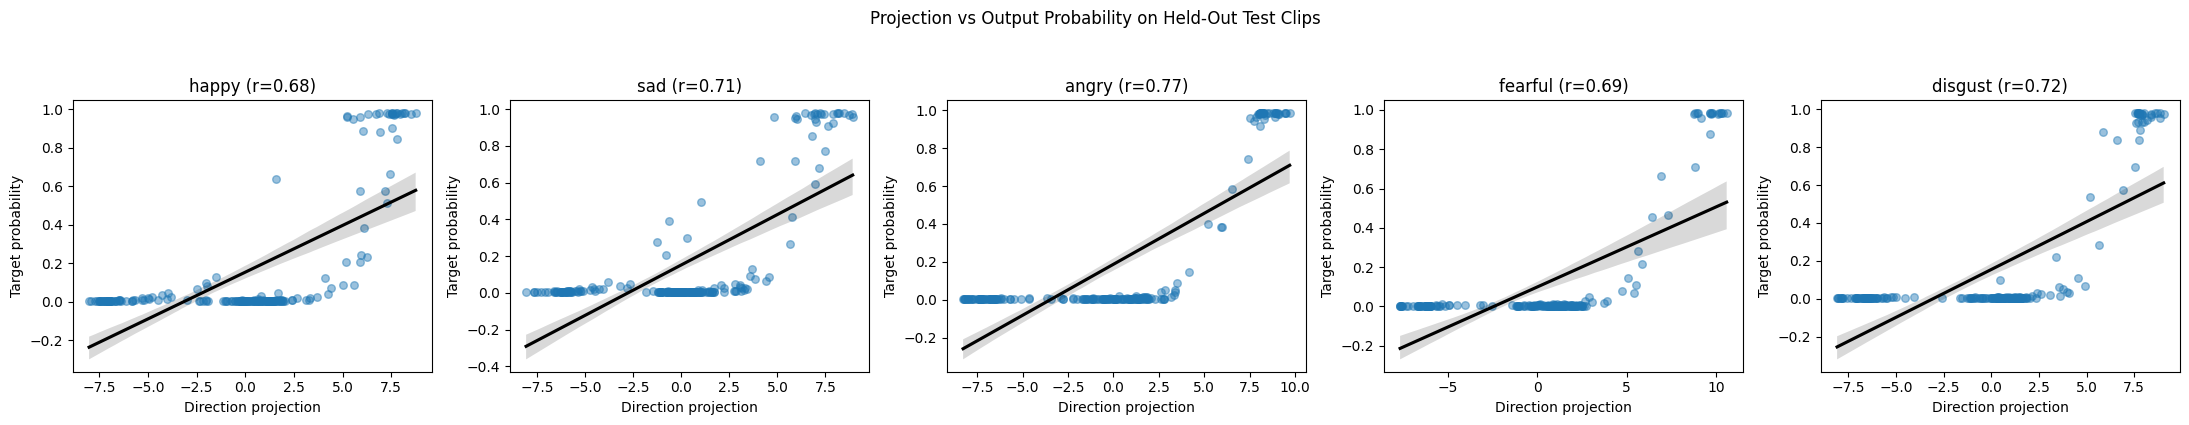
\includegraphics[width=\widefigwidth]{07_anthropic_style_emotion_vectors_cell_05_fig_02_anthropic_style_emotion_vector_analysis.png}
\caption{Projection onto each emotion direction correlates with the classifier probability for that emotion.}
\label{fig:projection_scatter}
\end{figure*}

This is the first bridge between internal geometry and class probabilities. The direction is not just a visualization axis; its scalar coordinate is aligned with the model's probabilistic output.

\subsection{Same-Context and Intensity Structure}

Same-speaker, same-sentence, same-repetition comparisons provide an especially clean test. When only emotion changes, the embedding displacement points in the expected emotion direction. Mean cosine to the expected direction ranges from 0.8203 to 0.9686 across non-neutral emotions. The intensity check adds a graded result: strong-intensity clips generally project farther along the same emotion direction than normal-intensity clips.

\section{Causal Direction Interventions}

\subsection{Steering and Ablation}

Final-layer steering adds or subtracts a learned direction from the pooled embedding before classification. At alpha 0.5, the mean target-probability increase is +0.1921 with bootstrap 95\% CI [0.1800, 0.2043]. Positive direction addition raises the corresponding emotion probability; negative direction addition suppresses it.

The complementary test removes components of embeddings along the learned emotion directions. Removing all non-neutral direction components drops macro F1 from 0.8237 to 0.5348, a delta of -0.2889 with 95\% CI [-0.3395, -0.2487].

\begin{figure}[t]
\centering
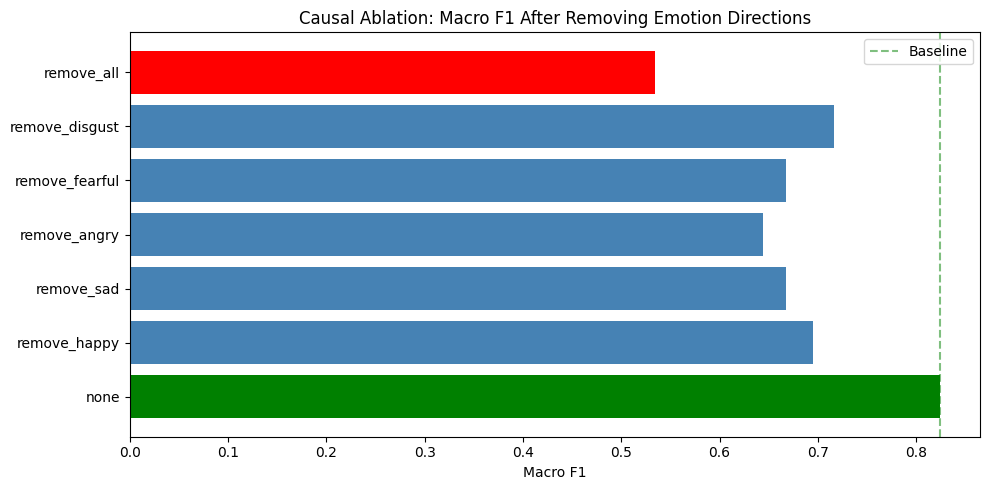
\includegraphics[width=\singlefigwidth]{09_causal_ablation_study_cell_06_fig_01_overall_ablation_results.png}
\caption{Final-embedding direction ablation damages classifier performance. Removing all emotion directions produces the largest drop.}
\label{fig:final_ablation}
\end{figure}

The random-direction control is decisive. Norm-matched random ablations have null mean 0.0002 and 95\% interval [0.0000, 0.0038], with fraction of null draws as damaging as the real ablation equal to 0.0. The ablation-strength sweep adds a dose-response view of the same necessity claim.

\begin{figure*}[t]
\centering
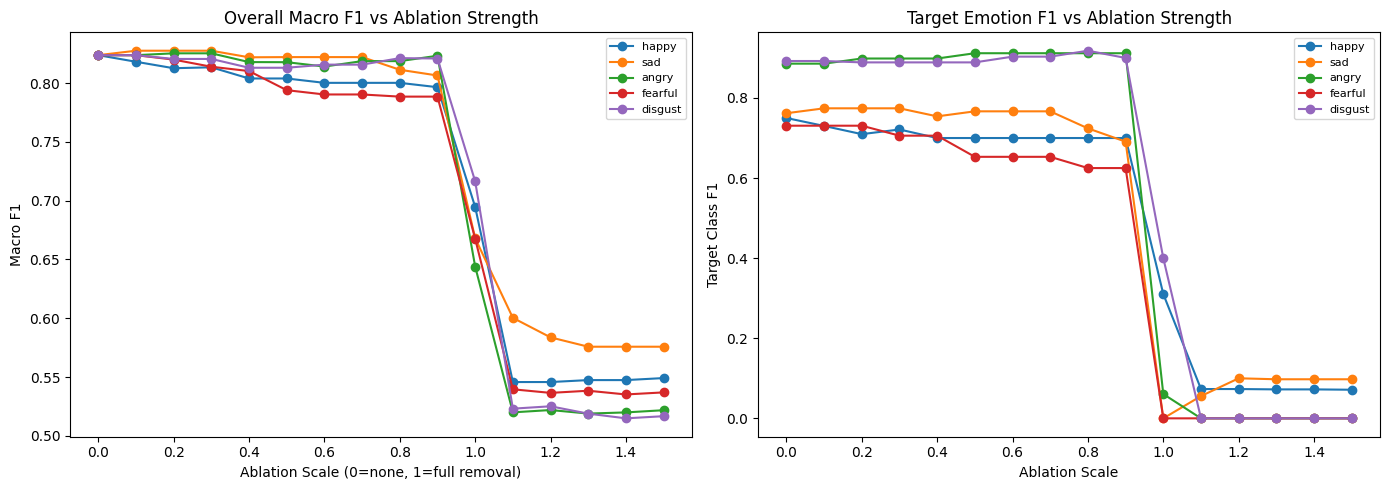
\includegraphics[width=\widefigwidth]{09_causal_ablation_study_cell_12_fig_04_ablation_strength_sweep.png}
\caption{Ablation-strength sweep. Performance remains stable under partial removal but drops sharply when the emotion-direction component is fully removed, showing that the learned directions are load-bearing rather than decorative.}
\label{fig:ablation_sweep}
\end{figure*}

\subsection{Mid-Transformer Causal Trace}

Final embedding interventions are useful, but they happen after most of the network has already computed. Notebook 14 upgrades the test by injecting and removing emotion directions inside wav2vec2 during the forward pass.

At each layer, layer-specific directions are added to hidden states at every valid time step, and the remaining transformer layers propagate naturally. The strongest average sufficiency effect occurs at layer 7, where alpha 0.5 increases target probability by +0.2545.

\begin{figure}[t]
\centering
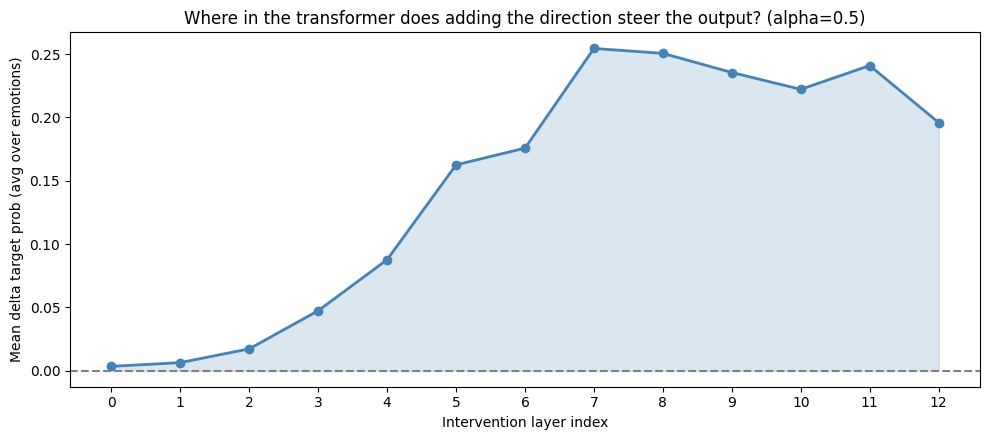
\includegraphics[width=\singlefigwidth]{14_mid_transformer_causal_intervention_cell_11_fig_02_3_experiment_1_mdash_mid_transformer_sufficiency_sweep.png}
\caption{Mid-transformer sufficiency by intervention layer. Direction injection is weak in early layers and becomes strongly causal in mid-to-late layers, peaking at layer 7.}
\label{fig:mid_sufficiency}
\end{figure}

A norm-matched random-vector injection control shows that this is not caused by generic hidden-state perturbation. For all target emotions, the fraction of random vectors matching or exceeding the real direction effect is 0.0.

\begin{figure}[t]
\centering
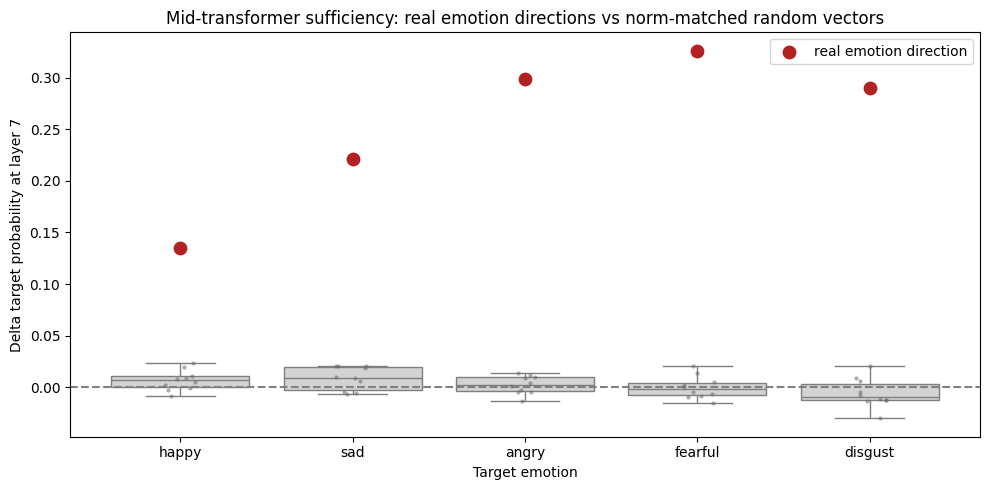
\includegraphics[width=\singlefigwidth]{14_mid_transformer_causal_intervention_cell_13_fig_03_3b_norm_matched_random_vector_sufficiency_control.png}
\caption{Random-vector sufficiency control. Real emotion directions produce larger effects than norm-matched random directions.}
\label{fig:mid_random}
\end{figure}

For necessity, direction removal inside the model is most damaging at layer 8, with average macro-F1 delta -0.1513. This is stronger than saying final embeddings contain separable clusters; it shows that emotion directions can be perturbed inside the model and still change the downstream output after the remaining layers run.

\section{Activation Patching with Real Clips}

Activation patching is the cleanest causal experiment in the project. Instead of adding a synthetic centroid direction, we patch a real hidden state from one clip into another. RAVDESS makes this possible because we can pair clips that share actor, sentence, repetition, and intensity but differ in emotion.

For an ordered source-destination pair, the destination hidden state at a selected layer is replaced with the source hidden state, and the rest of the model runs normally. If the destination prediction moves toward the source emotion, then the patched hidden state causally carries emotion identity.

The experiment evaluates 640 same-context ordered pairs at normal intensity. At layer 11, source-emotion probability increases by +0.6796 on average with 95\% CI [0.6475, 0.7092]; the argmax flips to the source emotion in 75.62\% of pairs with CI [72.19\%, 78.91\%].

\begin{figure*}[t]
\centering
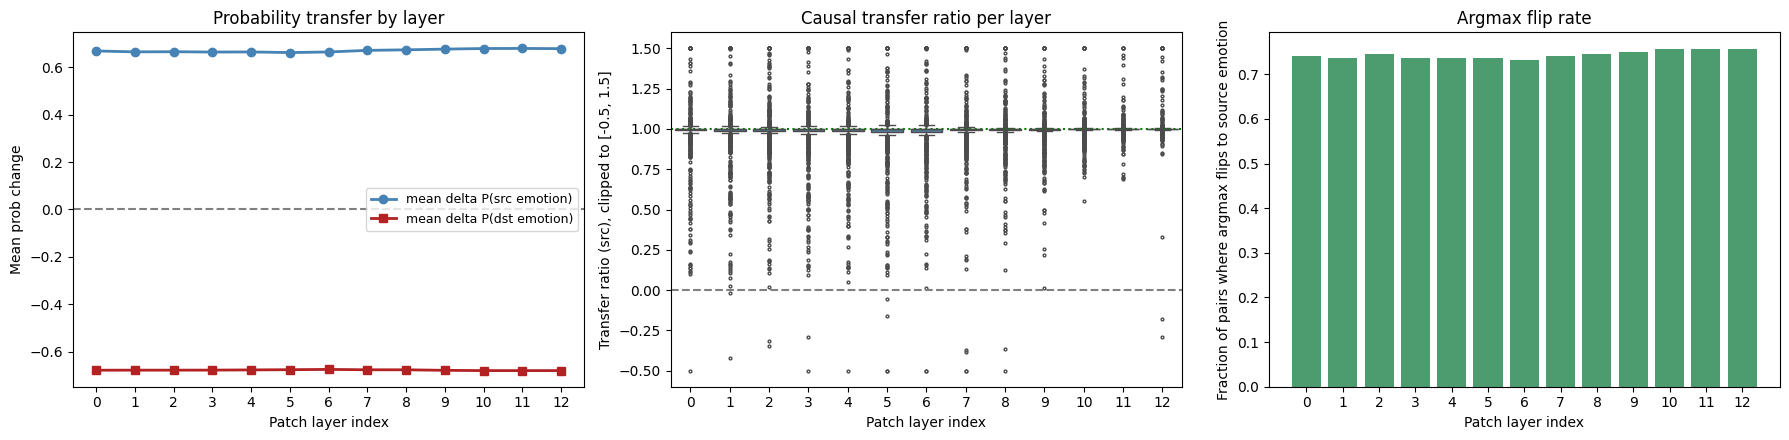
\includegraphics[width=\widefigwidth]{15_activation_patching_cell_13_fig_01_4_experiment_1_mdash_layer_wise_patch_transfer.png}
\caption{Activation patching transfers emotion identity. Replacing destination hidden states with source hidden states raises source-emotion probability and often flips the predicted class.}
\label{fig:patch_transfer}
\end{figure*}

\subsection{Direction Component vs Residual}

Notebook 15 decomposes the patch into a direction component and an orthogonal residual. This is the experiment that most directly links the vector story to real hidden-state mediation.

\begin{table}[t]
\caption{Patch Controls at Best Layer}
\label{tab:patch_controls}
\centering
\reporttablesize
\begin{tabular}{@{}lcc@{}}
\toprule
\textbf{Intervention} & \textbf{Delta P(src)} & \textbf{Flip} \\
\midrule
same-emotion different-context & +0.7328 & 0.8078 \\
full same-context patch & +0.6796 & 0.7562 \\
direction-component patch & +0.6395 & 0.7266 \\
orthogonal residual patch & +0.0533 & 0.1094 \\
self-patch control & +0.0002 & 0.0531 \\
random-source control & -0.0146 & 0.0406 \\
\bottomrule
\end{tabular}
\end{table}

\begin{figure*}[t]
\centering
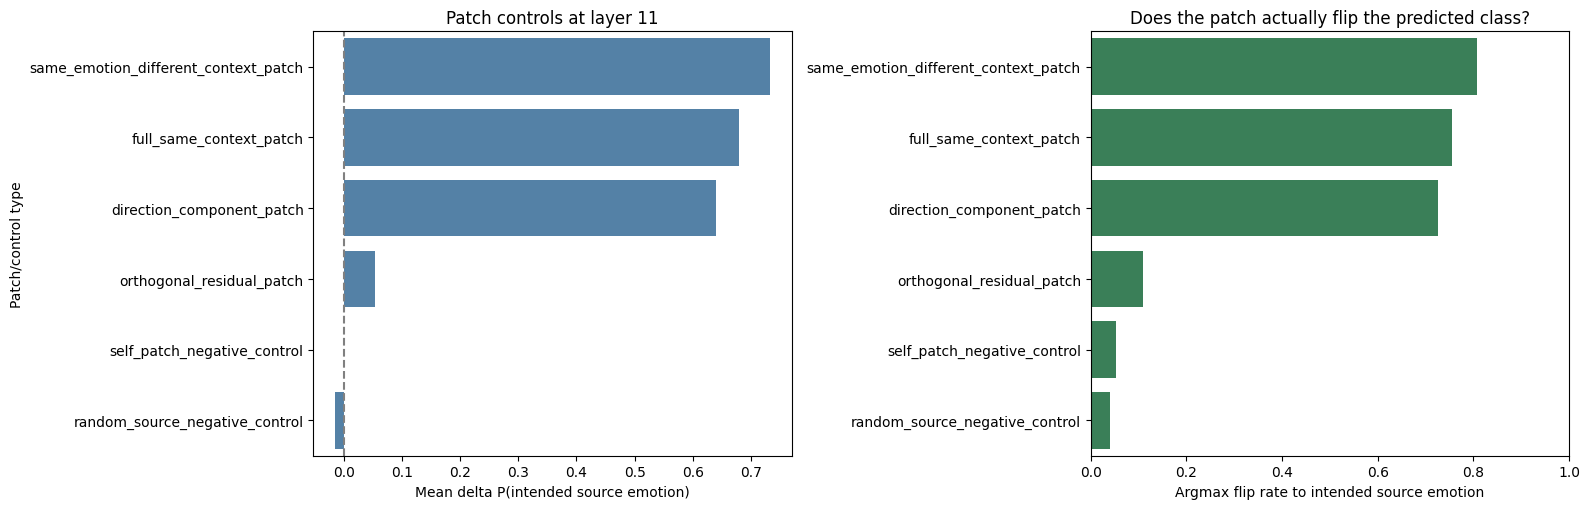
\includegraphics[width=\widefigwidth]{15_activation_patching_cell_27_fig_07_9_experiment_6_mdash_patch_controls_and_direction_component_decomposition.png}
\caption{Patch controls and direction-component decomposition. Most of the full patch effect is carried by the emotion-direction component, while negative controls fail.}
\label{fig:patch_controls}
\end{figure*}

The full hidden state transfers emotion strongly, and most of that transfer is carried by the emotion-direction component. The orthogonal residual is much weaker, while self-patch and random-source controls fail.

\subsection{Centroid Directions Are Powerful but Incomplete}

The project also avoids overclaiming. The pairwise patch effect and the synthetic centroid-direction steering effect are not strongly correlated at the individual pair level: Pearson $r=-0.0096$ and Spearman $r=-0.0629$.

\begin{figure*}[t]
\centering
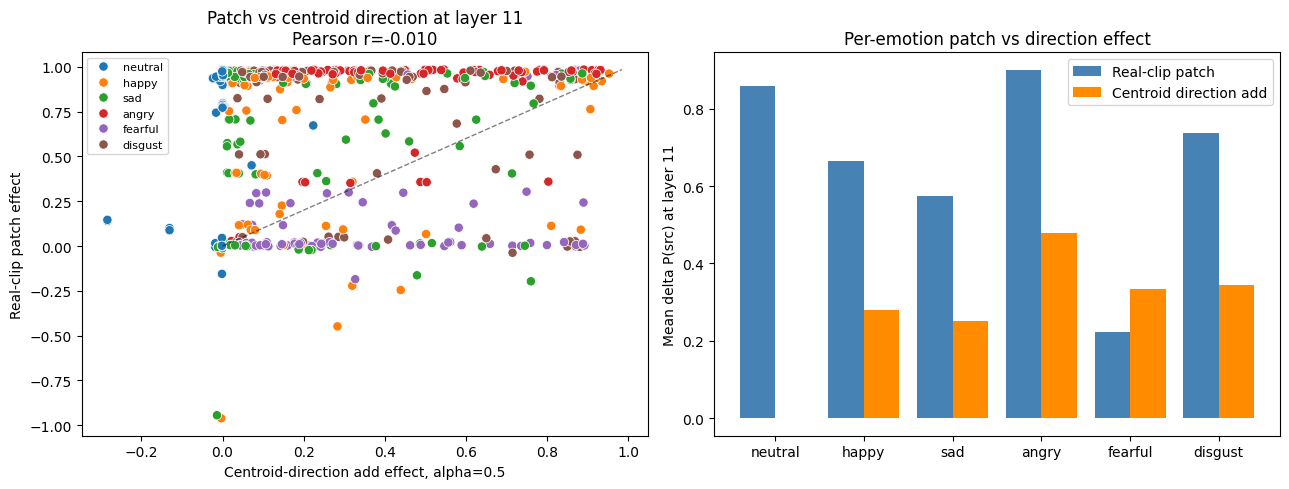
\includegraphics[width=\widefigwidth]{15_activation_patching_cell_17_fig_03_5_experiment_2_mdash_patch_effect_vs_centroid_direction_effect.png}
\caption{Real activation patches and centroid-direction additions do not strongly correlate pair by pair. Full hidden-state patches carry richer information than a single population-average direction.}
\label{fig:patch_vs_direction}
\end{figure*}

This refines the story. The model's internal emotion representation is not a single magic vector. Population directions are excellent probes and causal handles, but real examples contain richer high-dimensional structure: timing, speaker prosody, intensity, and pair-specific acoustic details. Pair-specific displacements become increasingly aligned with centroid contrasts in late layers, peaking at mean cosine 0.7490 in layer 12.

\section{Robustness and Boundaries}

Notebook 16 consolidates the statistical confidence story. The main findings survive bootstrap uncertainty, actor sensitivity checks, and null controls.

\begin{table}[t]
\caption{Bootstrap Confidence Intervals for Main Results}
\label{tab:cis}
\centering
\reporttablesize
\begin{tabular}{@{}lcc@{}}
\toprule
\textbf{Quantity} & \textbf{Point} & \textbf{95\% CI} \\
\midrule
trained head macro F1 & 0.8237 & [0.7688, 0.8762] \\
direction macro F1 & 0.8301 & [0.7703, 0.8796] \\
ablation F1 delta & -0.2889 & [-0.3395, -0.2487] \\
steering prob. delta & +0.1921 & [0.1800, 0.2043] \\
patch prob. delta & +0.6796 & [0.6475, 0.7092] \\
patch flip rate & 0.7562 & [0.7219, 0.7891] \\
\bottomrule
\end{tabular}
\end{table}

The per-test-actor analysis also matters. Actors 21--24 each have 52 test clips. Direction macro F1 ranges from 0.7677 to 0.8771, and ablation is damaging for every actor. This reduces the risk that one held-out actor is driving the result.

Cross-dataset transfer to CREMA-D \cite{cao2014cremad} is weak: trained-head macro F1 is 0.3498, centroid macro F1 is 0.3473, and direction-only macro F1 is 0.3444. This is an important boundary. The discovered geometry is strong for held-out RAVDESS speakers, but it is not a universal speech-emotion representation across datasets.

\section{Discussion}

The project now has a coherent causal chain. First, wav2vec2 learns speaker-independent emotion recognition much better than a conventional CNN baseline. Second, the final hidden space organizes emotion in directions that recover the classifier output. Third, projection magnitude tracks class probabilities. Fourth, adding or subtracting directions moves probabilities in the expected direction. Fifth, removing direction components damages performance, while norm-matched random directions do not. Sixth, injecting directions inside the transformer changes outputs after the remaining layers run. Seventh, real hidden-state patching transfers emotion identity between controlled clips, and the direction-component patch carries most of that transfer.

That is the Anthropic-inspired bridge. Anthropic studied emotion concepts in an LLM and showed that internal vectors could shape generated behavior. We study a speech classifier and show that internal emotion directions shape class probabilities. The output type is different, but the mechanistic structure is parallel: labeled emotional contexts produce vectors; projections align with behavior; interventions causally change outputs; and the interpretation is functional rather than subjective.

\subsection{How to Read the Evidence}

The most important distinction is between \emph{decodability} and \emph{causal use}. A representation is decodable if a probe or classifier can read information from it, but decodability alone does not prove the model relies on that information. Here, the direction-only classifier establishes decodability, while ablation, steering, mid-transformer intervention, and activation patching test causal use. When removing the direction hurts classification and adding the direction shifts probabilities, the representation is no longer merely readable; it is functionally connected to the output.

The negative controls make this causal claim more specific. Shuffled-label directions fail as classifiers, norm-matched random directions do not reproduce the ablation damage, and random-vector injections do not match real emotion-direction steering. The activation patching result then provides the closest speech analogue to Anthropic's behavioral intervention story: a real hidden state from one controlled clip transfers emotion evidence into another, and the direction-component patch carries most of that transfer. This is why the final conclusion is about a causal geometry rather than a single isolated vector.

\subsection{Do Models Have Emotions?}

This project should not claim that the model has emotions in the human, subjective, or conscious sense. A speech classifier does not feel anger when the angry probability increases. An LLM does not automatically have subjective fear because a fear vector activates.

The scientifically defensible claim is narrower and stronger: models can learn internal emotion-like variables that are functionally connected to behavior. In our case, the behavior is a predicted emotion distribution. The model's output is not only produced by a black-box classifier head; it is mediated by hidden-state geometry that can be probed and causally manipulated.

So the answer is: no, the model does not have emotions as experiences; yes, the model has manipulable internal representations corresponding to emotion concepts.

\section{Limitations}

RAVDESS is acted speech, not spontaneous affect. The results are about a model trained to classify acted emotional prosody. The speaker-independent split makes evaluation stronger, but the dataset is still small and controlled.

The directions are estimated from labeled training data, so the direction-only classifier is not external zero-shot recognition. It is better described as a direction-only prototype classifier.

The cross-dataset result is weak, so the learned geometry should be framed as robust inside the RAVDESS-style domain rather than universal across all emotional speech.

Activation patching replaces hidden-state sequences and can transfer more than emotion alone. The direction-component decomposition addresses this concern, but a deeper circuit-level project would need time-localized patching, path patching, and stronger disentanglement of prosody, speaker, and lexical content.

Finally, the project uses population centroid directions. These are useful and causal, but the low pairwise patch-vs-centroid correlation shows that individual examples contain richer structure than a single averaged vector.

\section{Conclusion}

The final project is complete as a data science and interpretability story. It starts with a standard SER model, but the strongest contribution is not simply classification accuracy. The stronger contribution is that emotion prediction in the model is linked to internal directions that are predictive, probabilistically aligned, causally steerable, necessary for performance, active inside the transformer, transferable through real activation patches, and robust against random/shuffled controls.

\begin{quote}
Emotion in this speech model is not a feeling; it is a causal geometry in hidden state space.
\end{quote}

That is the careful bridge between Anthropic's emotion-vector research and our RAVDESS wav2vec2 implementation. The model learns to predict emotion classes, but the prediction is mediated by internal emotion representations that can be experimentally tampered with to change the output.

\section*{Artifact Summary}

All notebooks from 01 through 16 executed with zero saved errors. Report figures and the Overleaf-ready source are preserved under \texttt{documentation/}, keeping the final narrative traceable to reproducible notebook artifacts rather than manually recreated plots.

\bibliographystyle{IEEEtran}
\bibliography{references}

\end{document}
